\documentclass[journal,12pt,onecolumn]{IEEEtran}
\usepackage{graphicx, float}
\graphicspath{{Figs/}}
\usepackage{multicol}
\usepackage{parskip}
\usepackage{titlesec}
\usepackage{color}
\usepackage{enumitem}
\usepackage{amsmath,amssymb,amsfonts,amsthm}
\usepackage{array}
\usepackage{booktabs}
\usepackage[table]{xcolor}
\usepackage{longtable}
\usepackage{gensymb}
\usepackage{cite}
\usepackage{algorithmic}
\usepackage{textcomp}
\usepackage{txfonts}
\usepackage{listings}
\usepackage{mathtools}
\usepackage{comment}
\usepackage{tkz-euclide}
\usepackage[breaklinks=true]{hyperref}
\usepackage{gvv}
\usepackage[latin1]{inputenc}
\usetikzlibrary{arrows.meta, positioning}
\usepackage{xparse}
\usepackage{calc}
\usepackage{multirow}
\usepackage{hhline}
\usepackage{ifthen}
\usepackage{lscape}
\usepackage{tabularx}
\usepackage{circuitikz}
\usepackage{tikz}
\newtheorem{problem}{Problem}
\newtheorem{theorem}{Theorem}[section]
\newtheorem{proposition}{Proposition}[section]
\newtheorem{lemma}{Lemma}[section]
\newtheorem{corollary}[theorem]{Corollary}
\newtheorem{example}{Example}[section]
\newtheorem{definition}[problem]{Definition}
\newcommand{\BEQA}{\begin{eqnarray}}
\newcommand{\EEQA}{\end{eqnarray}}
\theoremstyle{remark}

\title{GATE EY-2023 }
\author{AI25BTECH11016-VARUN}


\begin{document}

\maketitle
\textbf{Q.1 - Q.5 Carry ONE mark Each}

%1
\begin{enumerate}
    \item "You are delaying the completion of the task. Send  \underline{\hspace{1.5cm}}contributions at the
earliest."

\begin{enumerate}
\begin{multicols}{4}
\item you are
\item your
\item you're
\item yore

\end{multicols}
\end{enumerate}
\hfill{(GATE EY 2023)}

%2
 \item References :\underline{\hspace{1.5cm}} : : Guidelines : Implement

(By word meaning)
\begin{enumerate}
\begin{multicols}{4}
\item Sight
\item Site
\item Cite
\item Plagiarise

\end{multicols}
\end{enumerate}
\hfill{(GATE EY 2023)}

%3
 \item In the given figure, PQRS is a parallelogram with PS = 7 cm, PT = 4 cm and
PV = 5 cm. What is the length of RS in cm? (The diagram is representative.)
\begin{figure}[H]
    \centering
    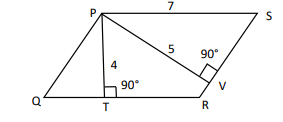
\includegraphics[]{figs/Q.3.png}
    \caption{}
    \label{fig:1}
\end{figure}
\begin{enumerate}
\begin{multicols}{4}
\item 20/7
\item 28/5
\item 9/2
\item 35/4

\end{multicols}
\end{enumerate}
\hfill{(GATE EY 2023)}

%4
 \item In 2022, June Huh was awarded the Fields medal, which is the highest prize in
Mathematics.
When he was younger, he was also a poet. He did not win any medals in the
International Mathematics Olympiads. He dropped out of college.
Based only on the above information, which one of the following statements can be
logically inferred with certainty?

\begin{enumerate}

\item Every Fields medalist has won a medal in an International Mathematics Olympiad
\item Everyone who has dropped out of college has won the Fields medal
\item All Fields medalists are part-time poets
\item Some Fields medalists have dropped out of college.


\end{enumerate}
\hfill{(GATE EY 2023)}

%5
 \item A line of symmetry is defined as a line that divides a figure into two parts in a way
such that each part is a mirror image of the other part about that line.
The given figure consists of 16 unit squares arranged as shown. In addition to the
three black squares, what is the minimum number of squares that must be coloured
black, such that both PQ and MN form lines of symmetry? (The figure is
representative)

\begin{figure}[H]
    \centering
    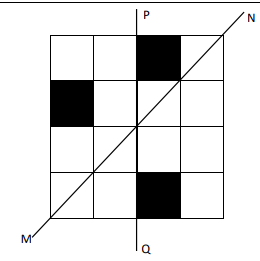
\includegraphics[]{figs/Q.5.png}
    \caption{}
    \label{fig:2}
\end{figure}
 
\begin{enumerate}
\begin{multicols}{4}
\item 3
\item 4
\item 5
\item 6

\end{multicols}
\end{enumerate}
\hfill{(GATE EY 2023)}


\textbf{Q.6 - Q.10 Carry TWO marks Each}
%6
 \item Human beings are one among many creatures that inhabit an imagined world. In
this imagined world, some creatures are cruel. If in this imagined world, it is given
that the statement "Some human beings are not cruel creatures" is FALSE, then
which of the following set of statement(s) can be logically inferred with certainty?

(i) All human beings are cruel creatures.

(ii) Some human beings are cruel creatures.

(iii) Some creatures that are cruel are human beings.

(iv) No human beings are cruel creatures.

\begin{enumerate}
\begin{multicols}{2}
\item only (i)
\item only (iii) and (iv)
\item only (i) and (ii)
\item only (i) and (ii)


\end{multicols}
\end{enumerate}
\hfill{(GATE EY 2023)}

%7
 \item To construct a wall, sand and cement are mixed in the ratio of 3:1. The cost of sand
and that of cement are in the ratio of 1:2.
If the total cost of sand and cement to construct the wall is 1000 rupees, then what
is the cost (in rupees) of cement used?

\begin{enumerate}
\begin{multicols}{4}
\item 400
\item 600
\item 800
\item 200

\end{multicols}
\end{enumerate}
\hfill{(GATE EY 2023)}
%8

 \item The World Bank has declared that it does not plan to offer new financing to Sri
Lanka, which is battling its worst economic crisis in decades, until the country has
an adequate macroeconomic policy framework in place. In a statement, the World
Bank said Sri Lanka needed to adopt structural reforms that focus on economic
stabilisation and tackle the root causes of its crisis. The latter has starved it of
foreign exchange and led to shortages of food, fuel, and medicines. The bank is
repurposing resources under existing loans to help alleviate shortages of essential
items such as medicine, cooking gas, fertiliser, meals for children, and cash for
vulnerable households.
Based only on the above passage, which one of the following statements can be
inferred with certainty?

\begin{enumerate}

\item According to the World Bank, the root cause of Sri Lanka's economic crisis is that
it does not have enough foreign exchange.
\item The World Bank has stated that it will advise the Sri Lankan government about how
to tackle the root causes of its economic crisis.
\item According to the World Bank, Sri Lanka does not yet have an adequate
macroeconomic policy framework.
\item The World Bank has stated that it will provide Sri Lanka with additional funds for
essentials such as food, fuel, and medicines.


\end{enumerate}
\hfill{(GATE EY 2023)}
%9
 \item The coefficient of $x^4$ in the polynomial $(x-1)^3(x-2)^3$ is equal to \underline{\hspace{1.5cm}}
\begin{enumerate}
\begin{multicols}{4}
\item 35
\item -3
\item 30
\item 21

\end{multicols}
\end{enumerate}
\hfill{(GATE EY 2023)}


 \item  Which one of the following shapes can be used to tile (completely cover by
repeating) a flat plane, extending to infinity in all directions, without leaving any
empty spaces in between them? The copies of the shape used to tile are identical
and are not allowed to overlap.
\begin{enumerate}
\begin{multicols}{4}
\item circle
\item regular octagon
\item regular pentagon
\item rhombus

\end{multicols}
\end{enumerate}

\hfill{(GATE EY 2023)}


\textbf{Q.11 - Q.35 Carry ONE mark Each}
 \item Which one of the following is an example of mechanical potential energy?
\begin{enumerate}
\begin{multicols}{2}
\item Activated neuron 
\item Polarized cell membrane
\item Stretched tendon
\item Relaxed muscle

\end{multicols}
\end{enumerate}

\hfill{(GATE EY 2023)}

 \item A research team studies the probability of crop damage by wild boar in crop
fields. For each crop field sampled, they record '1' if damage was observed, and
'0' if damage was not observed. Which one of the following distributions is most
appropriate to analyse the probability of crop damage?

\begin{enumerate}
\begin{multicols}{2}
\item Binomial distribution
\item Poisson distribution
\item Cauchy distribution
\item Gamma distribution

\end{multicols}
\end{enumerate}

\hfill{(GATE EY 2023)}
%13
 \item To test whether body size differs between two populations of a field mouse
species, a researcher measured 100 individuals in each population and calculated
the statistic
\[
\frac{\overline{X}_1 - \overline{X}_2}{S_p \sqrt{\tfrac{1}{n_1} + \tfrac{1}{n_2}}}
\]
where $\overline{X}_1$ and $\overline{X}_2$ are the mean body sizes of the two populations,
respectively, $S_p$ is the pooled standard deviation, and $n_1$ and $n_2$ are the sample sizes
for the two populations, respectively.

This statistic is used in the

\begin{enumerate}
\begin{multicols}{4}
\item Chi-square test
\item Kruskal-Wallis test
\item Student's t-test
\item Mann-Whitney U test

\end{multicols}
\end{enumerate}
\hfill{(GATE EY 2023)}

%14

 \item Which one of the following ecological processes best explains the observation that
seedling establishment increases with distance from the parent tree in a forest?

\begin{enumerate}

\item Competition between species
\item Competition within species

\item Facilitation between species

\item Facilitation within species


\end{enumerate}

\hfill{(GATE EY 2023)}

%15
 \item In the early 20th century, which one of these scientists made fundamental
contributions to both the fields of evolution and statistics?
\begin{enumerate}
\begin{multicols}{2}
\item R. A. Fisher
\item Niko Tinbergen
\item August Weismann
\item Thomas Huxley

\end{multicols}
\end{enumerate}

\hfill{(GATE EY 2023)}
%16

 \item The figure depicts how body temperature changes for two species (L and M) as a
function of ambient temperature. 

\begin{figure}[H]
    \centering
    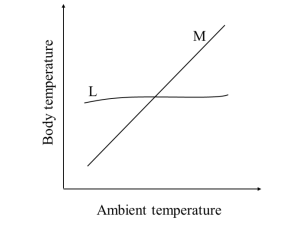
\includegraphics[]{figs/Q.16.png}
    \caption{}
    \label{fig:3}
\end{figure}
Which one of the following statements about how L and M regulate temperature is
correct?
\begin{enumerate}

\item L and M are both homeotherms.
\item L and M are both homeotherms.
\item L is a homeotherm, whereas M is a poikilotherm.
\item L is a poikilotherm, whereas M is a homeotherm.


\end{enumerate}

\hfill{(GATE EY 2023)}
%17
 \item You are a deep-sea organism and your potential mates are several hundreds of
kilometers away from you. Which one of the following kinds of mating signals is
most likely to help them locate you?
\begin{enumerate}
\begin{multicols}{2}
\item Display gestures
\item Electric pulses
\item Body colouration
\item Sounds


\end{multicols}
\end{enumerate}


\hfill{(GATE EY 2023)}

%18
 \item Which one of the following options represents the correct order with respect to
levels of organization?
B - biomes; E - ecosystems; P - populations; I - individuals; C - communities
\begin{enumerate}
\begin{multicols}{4}
\item $I < P < C < E < B$
\item $I < C < P < E < B$
\item $I < E < C < P < B$
\item $I < P < E < C < B$

\end{multicols}
\end{enumerate}


\hfill{(GATE EY 2023)}


%19
 \item Which one of the following options describes the difference between abiotic
resources and abiotic conditions?
\begin{enumerate}

\item Resource levels can fluctuate but conditions do not.
\item Conditions can fluctuate but resource levels do not
\item Resources can be used up by organisms, whereas conditions cannot.
\item Conditions can be used up by organisms, whereas resources cannot


\end{enumerate}


\hfill{(GATE EY 2023)}

%20
 \item Which one of the following ranges correctly represents the percentage of energy
that is transferred from a lower to the next higher trophic level in most terrestrial
systems?
\begin{enumerate}
\begin{multicols}{4}
\item 0.01 \% to 1 \%
\item 33 \% to 66 \%
\item 2 \% to 20 \%

\item 90 \% to 95 \%

\end{multicols}
\end{enumerate}

\hfill{(GATE EY 2023)}


%21


 \item Whales and dolphins are hypothesized to have evolved along the northern shore of
the Tethys Sea, prior to the Indian plate's collision with the Eurasian plate. To
which one of the following animals are these aquatic mammals most closely
related?
\begin{enumerate}
\begin{multicols}{4}
\item pigs
\item elephants
\item seals
\item zebras

\end{multicols}
\end{enumerate}

\hfill{(GATE EY 2023)}


%22

 \item Which one of the following options represents the correct order of decreasing
average net primary productivity (g/m2
/ year) in natural ecosystems?
\begin{enumerate}

\item Swamp and marshes $>$ Tropical forests $>$  Temperate forests $>$  Temperate
grasslands $>$  Tundra
\item Swamps and marshes $>$  Tropical forests $>$  Temperate forests $>$  Tundra $>$ 
Temperate grasslands 
\item Tropical forests $>$  Swamps and marshes $>$  Temperate forests $>$  Tundra $>$ 
Temperate grasslands
\item Tropical forests $>$  Swamps and marshes $>$  Temperate forests $>$  Temperate
grasslands $>$  Tundra


\end{enumerate}


\hfill{(GATE EY 2023)}


%23

 \item 
 The increase in mean global temperature since the industrial revolution falls in the
range of
\begin{enumerate}
\begin{multicols}{4}
\item $0^\circ\text{C to }0.5^\circ\text{C}$

\item $0.5^\circ\text{C to }2^\circ\text{C}$

\item $2^\circ\text{C to }5^\circ\text{C}$

\item $>5^\circ\text{C}$


\end{multicols}
\end{enumerate}

\hfill{(GATE EY 2023)}




 \item Which one of the following endangered species has been the subject of a
reintroduction plan in India?
\begin{enumerate}
\begin{multicols}{4}
\item Rusty spotted cat
\item Jungle cat
\item Cheetah
\item Jaguar

\end{multicols}
\end{enumerate}



\hfill{(GATE EY 2023)}



 \item Compared with bony fish, many shark species show steeper population declines in
response to heavy fishing pressure. Which one of the following options explains
this?

\begin{enumerate}

\item Sharks are dangerous to humans
\item Sharks evolved over 400 million years ago.
\item Sharks are long lived and late maturing
\item Sharks are only found in open oceans


\end{enumerate}



\hfill{(GATE EY 2023)}


 \item Which one or more of the following options describe(s) how ferns differ from
angiosperms and gymnosperms?
\begin{enumerate}

\item Ferns lack a vascular system
\item Ferns have separate haploid and diploid generations.
\item Ferns are pollinated by flies
\item Ferns are known only from the fossil record


\end{enumerate}


\hfill{(GATE EY 2023)}




 \item The IUCN Red List is based on a set of criteria to evaluate species vulnerability to
extinction. Which one or more of the options is/are used as criteria?
\begin{enumerate}
\begin{multicols}{2}
\item Absolute population size
\item Geographic range
\item Economic value
\item Change in population size over time


\end{multicols}
\end{enumerate}

\hfill{(GATE EY 2023)}





 \item Which one or more of the following processes contribute(s) substantially to
increased mean global temperatures?

\begin{enumerate}

\item Decreased greenhouse gases in the atmosphere
\item Increased tropical deforestation
\item Decreased methane emissions
\item Increased fossil fuel use


\end{enumerate}
\hfill{(GATE EY 2023)}


%29


 \item Depending on soil nutrient availability, which one or more of the following
interaction(s) can occur between soil mycorrhizal fungi and plants?

\begin{enumerate}
\begin{multicols}{4}
\item Parasitism
\item Predation
\item Mutualism
\item Commensalism


\end{multicols}
\end{enumerate}

\hfill{(GATE EY 2023)}


%30

 \item Which one or more of the following is/are characteristic of r-selected animals?
\begin{enumerate}

\item They have a long lifespan.
\item They produce a large number of offspring in each reproductive event
\item They produce a few large bodied offspring in each reproductive event
\item They reproduce at a young age.


\end{enumerate}


\hfill{(GATE EY 2023)}
%31

 \item Which one or more of the following represent(s) benefits of Batesian mimicry to
the mimic?

\begin{enumerate}

\item Increased toxicity against potential predators

\item Reduced cooperation
\item Increased protection from predators without investment in toxicity
\item Reduced competition



\end{enumerate}

\hfill{(GATE EY 2023)}

%32

 \item Which one or more of the following is/are developmental feature(s) of hatchlings
of an altricial bird species?
\begin{enumerate}
\begin{multicols}{2}
\item Eyes open 
\item Eyes closed 
\item Down feathers present
\item Down feathers absent

\end{multicols}
\end{enumerate}
\hfill{(GATE EY 2023)}


%33


 \item You have a biased coin with the probability of getting a head being 0.6. The
probability of getting at least 1 head in 3 tosses is \underline{\hspace{1.5cm}}.
(Rounded off to three decimal places)

\hfill{(GATE EY 2023)}

%34

 \item A lake has 20 blue male, 30 red male, 60 blue female and 80 red female fish. A
researcher catches one individual at random from the lake. If the caught fish is
blue, the probability that it is female is \underline{\hspace{1.5cm}}
(Rounded off to two decimal places)
\hfill{(GATE EY 2023)}

%35


 \item A researcher fitted a function to data on how foraging rate (F, number of items
consumed per 10 minutes) of a shorebird varied with its group size (G, number of
individuals) and obtained the following equation:
\[
\log_{e} F = 3 - 0.2 \times \log_{e} G
\]

According to this equation, the foraging rate (F) of a solitary forager is
\underline{\hspace{1.5cm}} items per 10 minutes.
(Rounded off to the nearest integer)
\hfill{(GATE EY 2023)}
\textbf{Q.36 - Q.65 Carry TWO marks Each}
%36

 \item 
 Two species of birds, A and B, are found together in region X. Only species A is
present in region Y. Both species produce species-specific alarm calls in response
to a predator P. A researcher conducts experiments where she plays recorded calls
of both species to species A in regions X and Y. The response of species A to the
recorded calls are summarized in the table below.

\begin{table}[h!]
\centering
\begin{tabular}{|l|l|l|}
\hline
\textbf{Call stimulus} & \textbf{Response in region X} & \textbf{Response in region Y} \\ \hline
Alarm call of species A & Species A flies for cover & Species A flies for cover \\ \hline
Alarm call of species B & Species A flies for cover & Species A does not respond \\ \hline
\end{tabular}
\end{table}


Based on the results, the most appropriate inference is that
\begin{enumerate}

\item species A's response to species B's alarm call is a learned behavior
\item species A's response to species B's alarm call is an innate behavior
\item predator P is absent in region Y.
\item predator P exclusively preys on species B


\end{enumerate}

\hfill{(GATE EY 2023)}

%37

 \item The table below lists different insects and taxonomic orders. Choose the option
that matches the animal to its correct taxonomic order

\begin{table}[h!]
\centering
\begin{tabular}{|l|l|}
\hline
\textbf{Animal} & \textbf{Taxonomic order} \\ \hline
P) Moths        & i) Hemiptera     \\ \hline
Q) True bugs    & ii) Orthoptera   \\ \hline
R) Crickets     & iii) Coleoptera  \\ \hline
S) Beetles      & iv) Lepidoptera  \\ \hline
                & v) Diptera       \\ \hline
\end{tabular}
\end{table}



\begin{enumerate}

\item P-ii; Q-i; R-v; S-iv
\item P-iii; Q-v; R-iv; S-i
\item P-iv; Q-i; R-ii; S-iii
\item P-iv; Q-ii; R-i; S-v


\end{enumerate}
\hfill{(GATE EY 2023)}

%38
 \item Islands I, II, and III lie off a mainland coast. Which one of the following
statements about species richness is consistent with the theory of island
biogeography?


\begin{figure}[H]
    \centering
    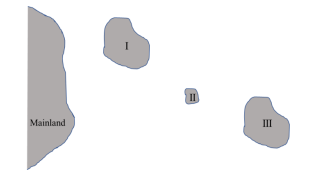
\includegraphics[]{figs/Q.38.png}
    \caption{}
    \label{fig:4}
\end{figure}
\begin{enumerate}

\item Island II has the highest species richness because it has the lowest area.
\item Island III has the highest species richness because it is large and farthest from the
mainland.
\item Island I has the highest species richness because it is large and closest to the
mainland.
\item Islands I and III have equally high species richness because they have roughly the
same area


\end{enumerate}
\hfill{(GATE EY 2023)}


%39

 \item In a polygynous hummingbird species, males defend and monopolize nectar-rich
plants (resource). Females visit these plants for nectar and the defending male will
have access to all visiting females for mating. Under which scenario is polygyny
expected to be the highest?
\begin{enumerate}

\item Resources are abundant and evenly distributed
\item Resources are abundant and clumped
\item Resources are scarce and evenly distributed
\item Resources are scarce and randomly distributed


\end{enumerate}



\hfill{(GATE EY 2023)}


%40
 \item A researcher estimates the relationship between reproductive success ($N$, number
of offspring) and horn length ($H$, in cm) in a wild goat as
$N$= 40 -2.2$H$ + 0.04$H^2$
Horn length typically varies from 10 cm to 50 cm in this species. Which one of the
following graphs correctly represents this relationship?
\begin{figure}[H]
    \centering
    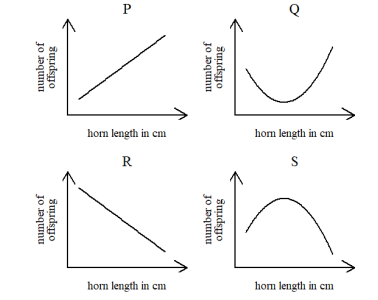
\includegraphics[]{figs/Q.40.png}
    \caption{}
    \label{fig:5}
\end{figure}
   
\begin{enumerate}
\begin{multicols}{4}
\item P
\item Q
\item R
\item s

\end{multicols}
\end{enumerate}


\hfill{(GATE EY 2023)}



%41

 \item Overfishing reduced food availability for sea lions in California, causing a decline
in their population size. In 1972, under the US Endangered Species Act, fishing
was banned from sea lion foraging areas. Subsequently, the population of sea lions
increased in a logistic form as shown in the figure. 

\begin{figure}[H]
    \centering
    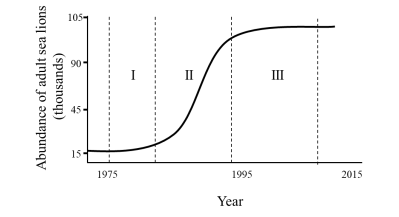
\includegraphics[]{figs/Q.41.png}
    \caption{}
    \label{fig:6}
\end{figure}
   
The per capita growth rate is highest in the interval \underline{\hspace{1.5cm}} and the population
growth rate is highest in the interval\underline{\hspace{1.5cm}} . 
\begin{enumerate}
\begin{multicols}{4}
\item I, II
\item I, III
\item II, II
\item III,II

\end{multicols}
\end{enumerate}



\hfill{(GATE EY 2023)}

%42
 \item A locus at Hardy-Weinberg equilibrium in a diploid organism has n alleles. The
maximum heterozygosity (i.e., proportion of heterozygotes) for this locus is
\begin{enumerate}
\begin{multicols}{4}
\item $n$ 
\item $1/n$
\item $1-(1/n)$
\item $1-n$

\end{multicols}
\end{enumerate}


\hfill{(GATE EY 2023)}
%43

 \item Match the diseases to the pathogens that cause them.
\begin{table}[h!]
\centering
\begin{tabular}{|l|l|}
\hline
\textbf{Diseases} & \textbf{Pathogens} \\ \hline
P) Avian malaria          & i) Virus \\ \hline
Q) COVID-19 in humans     & ii) \textit{Plasmodium} \\ \hline
R) Chytrid disease in frogs & iii) Mosquito \\ \hline
                         & iv) Fungus \\ \hline
\end{tabular}
\end{table}


\begin{enumerate}
\begin{multicols}{4}
\item P-i; Q-iii; R-iv
\item P-iii; Q-i; R-ii
\item P-ii; Q-i; R-iv
\item P-iv; Q-i; R-ii

\end{multicols}
\end{enumerate}

\hfill{(GATE EY 2023)}

%44
 \item The production of anthocyanin pigments in pea flowers requires the presence of
at least one dominant allele in each of two independently assorting genes, C and P.
The presence of anthocyanin results in purple flowers, whereas its absence gives
white flowers. A cross between two double heterozygous (CcPp) plants is
performed. What is the expected ratio of plants with purple flowers to plants with
white flowers?
\begin{enumerate}
\begin{multicols}{4}
\item 1:3
\item 3:1
\item 5:3
\item 9:7

\end{multicols}
\end{enumerate}

\hfill{(GATE EY 2023)}

%45


 \item In the phylogenetic trees shown, the tips represent different species of geckos
(labeled A to E) and the areas to which they belong. Which one of these is most
consistent with the hypothesis that the geckos colonized the Western Ghats from
Northeast India through the Eastern Ghats?
\begin{figure}[H]
    \centering
    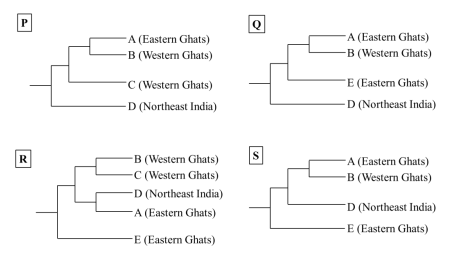
\includegraphics[]{figs/Q.45.png}
    \caption{}
    \label{fig:7}
\end{figure}
\begin{enumerate}
\begin{multicols}{4}


\item P
\item Q
\item R
\item S

\end{multicols}
\end{enumerate}


\hfill{(GATE EY 2023)}

%46
 \item The phylogenetic tree depicts the relationship between 5 species of snakes
(labelled A to E) and provides information about their habitat specialization.
Given the principle of parsimony (least number of evolutionary changes required)
and that ancestor Y was terrestrial, which one of the options given is correct?
\begin{figure}[H]
    \centering
    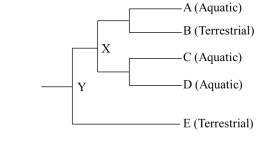
\includegraphics[]{figs/Q.46.png}
    \caption{}
    \label{fig:}
\end{figure}
\begin{enumerate}

\item X was more likely to be aquatic than terrestrial
\item X was more likely to be terrestrial than aquatic.
\item X was equally likely to be aquatic or terrestrial.

\item X was neither aquatic nor terrestrial.


\end{enumerate}


\hfill{(GATE EY 2023)}


%47
 \item The mode of speciation in snakes in the Western Ghats is predominantly allopatric.
A researcher wants to quantify diversification of snakes in this range. From the
options given, choose the most cost and time efficient way to sample snakes.
\begin{enumerate}

\item Across an elevational gradient
\item Across barriers such as valleys and rivers
\item Intensively in one or two random locations
\item Intensively across the entire mountain range


\end{enumerate}
\hfill{(GATE EY 2023)}

%48


 \item
 All else being equal, which one of the following population sizes $(N)$ and 
migration rates $(m)$ would result in the most genetic differentiation between 
populations ($F_{st}$)?

Note that $F_{st}$ is computed as
\[
F_{st} = \frac{1}{4Nm + 1}
\]

\begin{enumerate}
\begin{multicols}{2}
\item $N$=500,$m$=1
\item $N$=200,$m$=200
\item $N$=40,$m$=10
\item $N$40,$m$=1

\end{multicols}
\end{enumerate}
\hfill{(GATE EY 2023)}


%49


 \item Which one or more of the following is/are prediction(s) or assumption(s) of the
handicap principle for the evolution of sexual signals?
\begin{enumerate}

\item Females prefer costly signals.
\item Honest signals are costly to produce.
\item Males displaying costly signals are not chosen by females.
\item Costly signals are reliable indicators of signaller quality.


\end{enumerate}

\hfill{(GATE EY 2023)}


%50

 \item A research team assesses the impact of the invasive species Lantana camara on the
seed set of a native flowering plant S. The plant S usually grows in clumps with
other individuals of the same or different flowering species. They measure the seed
set of flowering individuals of S grown (i) alone; (ii) with a conspecific (same
species); (iii) with a native species Q; (iv) with a native species R; (v) with
Lantana camara. The figure below shows the mean seed set with 95 \% confidence
intervals for the different treatments. 
\begin{figure}[H]
    \centering
    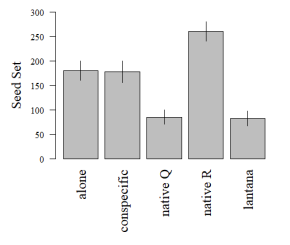
\includegraphics[]{figs/Q.50.png}
    \caption{}
    \label{fig:9}
\end{figure}

Based on the figure provided, which one or more of the options given is/are
correct?

\begin{enumerate}

\item Seed set is higher in the presence of both the native species than in the presence of
a conspecific.

\item Seed set is lower in the presence of Lantana camara than in the presence of both
the native species.
\item Seed set is lower in the presence of Lantana camara than in the presence of a
conspecific.
\item Seed set is always higher in the presence of other plants than when grown alone


\end{enumerate}
\hfill{(GATE EY 2023)}

%51


 \item There are two palatable prey species, Q and R, for an insectivorous bird species in
a forest. However, the bird searches for and consumes only species Q. According
to optimal foraging theory, which one or more of the following conditions can
explain the bird choosing to forage only for Q?

\begin{enumerate}

\item The handling time for Q $>$ the handling time of R
\item The handling time for Q $<$ the handling time of R
\item The relative abundance of Q $>$ the relative abundance of R
\item The relative abundance of Q $<$ the relative abundance of R


\end{enumerate}

\hfill{(GATE EY 2023)}


 \item Conservation biologists have debated whether protected areas should be designed
as a single large patch or as several small patches. Assuming that the total area is
the same for the two designs, which one or more of the options describe(s) the
conservation benefit(s) of several small patches?
\begin{enumerate}

\item Lower rates of local extinction
\item Lower rates of diversification
\item Lower spread of disease across the populations
\item Lower population size


\end{enumerate}
\hfill{(GATE EY 2023)}

%53

 \item Which one or more options is/are example(s) of niche partitioning between
species?

\begin{enumerate}
\begin{multicols}{2}
\item Temporal separation of activity
\item Diet specialization
\item Hybridization
\item Vertical stratification of foraging heights

\end{multicols}
\end{enumerate}

\hfill{(GATE EY 2023)}

%54


 \item
  In an assemblage of coexisting wild cat species, the size of canine teeth was found
to be strikingly different between these species. Which one or more of the
following statements explain(s) this observation? 
\begin{enumerate}

\item Differences in the size of canine teeth were driven by the size of prey captured by
the different species.
\item Differences in the size of canine teeth are an example of divergent evolution
\item Differences in the size of canine teeth are an example of convergent evolution.

\item Differences in the size of canine teeth were driven by past competition


\end{enumerate}
\hfill{(GATE EY 2023)}


%55

 \item The Biological Species Concept (BSC) states that 'species are groups of
interbreeding natural populations that are reproductively isolated from other such
groups'. Which one or more of the options could pose challenges for defining
species using the BSC?
\begin{enumerate}
\begin{multicols}{2}
\item Fertile interspecies hybrids 
\item Extinct fossil species
\item Barriers to gene flow
\item Barriers to gene flow

\end{multicols}
\end{enumerate}


\hfill{(GATE EY 2023)}

%56

 \item The barnacle species, Chthamalus stellatus (CS), is found only in the high
intertidal zone whereas Balanus glandula (BG) is found only in the low intertidal
zone. A researcher transplanted CS from the high to low (T-CS), and BG from the
low to high (T-BG) intertidal zones. Additionally, they allowed the species to grow
alone or in competition with each other, and quantified survival.
Which one or more of the following inferences is/are consistent with the
experimental results shown below?

\begin{figure}[H]
    \centering
    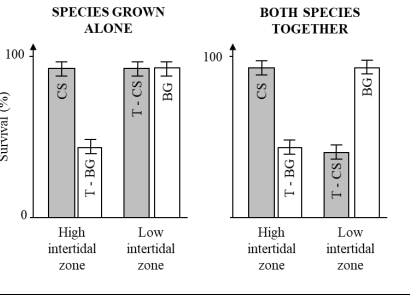
\includegraphics[]{figs/Q.56.png}
    \caption{}
    \label{fig:10}
\end{figure}

\begin{enumerate}

\item Only abiotic conditions increase mortality of BG in the high intertidal zones.
\item Only abiotic conditions increase mortality of CS in the low intertidal zones.
\item Interspecific competition increases mortality of BG in the high intertidal zon
\item Interspecific competition increases mortality of CS in the low intertidal zone


\end{enumerate}


\hfill{(GATE EY 2023)}


%57
 \item 
 In the figure below, ellipse X represents the combinations of salt concentrations
and temperatures that a marine invertebrate species can tolerate. Ellipse Y
represents the combinations of salt concentrations and temperatures that this
species is actually found in.
\begin{figure}[H]
    \centering
    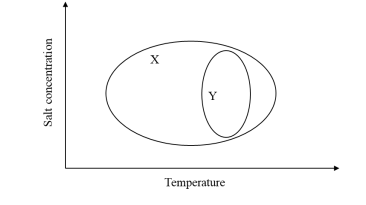
\includegraphics[]{figs/Q.57.png}
    \caption{}
    \label{fig:11}
\end{figure}
Which one or more of the following statements about X and Y is/are correct?
\begin{enumerate}

\item X is the fundamental niche of the species, whereas Y is the realized niche.
\item The difference between X and Y can result from biotic interactions.
\item The difference between X and Y can result from dispersal limitation
\item The difference between X and Y results from the species' tolerance to salt
concentrations.


\end{enumerate}

\hfill{(GATE EY 2023)}

%58



 \item A butterfly species inhabits four types of patchy landscapes (P, Q, R, S). Grey
shapes represent occupied habitat and white shapes are unoccupied. Arrows
represent the occurrence and directions of possible dispersal. 

\begin{figure}[H]
    \centering
    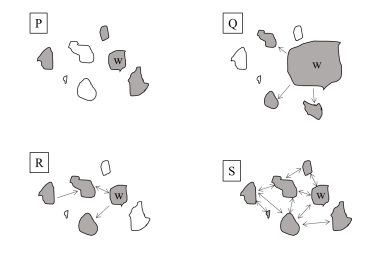
\includegraphics[]{figs/Q.58.png}
    \caption{}
    \label{fig:}
\end{figure}
Which one or more of the options is/are likely to be correct?
\begin{enumerate}

\item In landscape Q, patch w is a source population
\item Landscape R represents a metapopulation.
\item Landscape P has the highest extinction rate.
\item Landscape S has the highest level of inbreeding.


\end{enumerate}

\hfill{(GATE EY 2023)}

%59

 \item A new food requesting behaviour has been observed in bonnet macaques in
Bandipur National Park. The macaques extend their hand and make a cooing sound
only towards humans, which effectively results in food given to them. If this
behaviour is to increase in frequency in the population over time by the process of
natural selection, which one or more of the options below is/are necessary
condition(s)? 
\begin{enumerate}

\item Food requesting behaviour must be transmitted from one generation to the next.
\item All bonnet macaques in the area must show this behaviour.
\item Macaques who receive food using this behaviour are able to have more offspring.
\item Food requesting behaviour must only be taught by parents to offspring.


\end{enumerate}


\hfill{(GATE EY 2023)}
%60

 \item Two co-occurring plant species, A and B, flower at the same time. They are visited
by the same pollinator species. If these plants are pollinator-limited, then which
one or more of the following statements is/are correct with regard to the figure
shown below?

\begin{figure}[H]
    \centering
    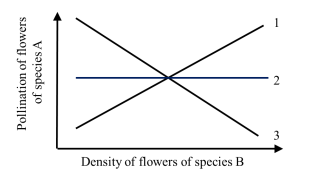
\includegraphics[]{figs/Q.60.png}
    \caption{}
    \label{fig:}
\end{figure}
\begin{enumerate}

\item Line 1 represents competition.
\item Line 2 represents mutualism.
\item Line 3 represents parasitism.
\item Line 1 represents facilitation


\end{enumerate}


\hfill{(GATE EY 2023)}

%61

 \item Scorpions on the sand dunes in Syria in September 2022 have the age distribution
as shown in Figure P. Scorpions can live to a maximum of 90 days. In all the
figure panels, the x-axis represents age class and the y-axis represents number of
individuals.
Assuming no immigration or emigration, which one or more of the age distribution
panels Q, R, S, T is/are possible 30 days later?

\begin{figure}[H]
    \centering
    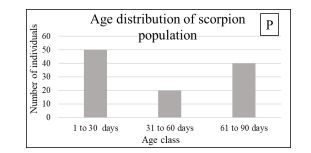
\includegraphics[]{figs/Q.61.png}
    \caption{}
    \label{fig:14}
   \end{figure} 
    \begin{figure}[H]
    \centering
    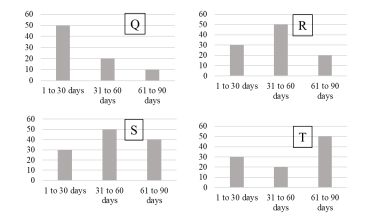
\includegraphics[]{figs/O.61.png}
    \caption{}
    \label{fig:14}
\end{figure}
\begin{enumerate}
\begin{multicols}{4}
\item Q
\item R
\item S
\item T

\end{multicols}
\end{enumerate}
\hfill{(GATE EY 2023)}


%62


 \item The Shannon-Weaver index $H$ is a measure of diversity and is calculated as  

\[
H = - \sum_{i=1}^{S} p_i \ln(p_i)
\]

where $S$ is the total number of species and $p_i$ is the proportional abundance of a species $i$.

The table below gives the abundance of different species in a community. The
Shannon-Weaver index of reptile diversity in this community is\underline{\hspace{1.5cm}}.
(Rounded off to two decimal places)
\begin{table}[h!]
\centering
\begin{tabular}{|l|c|}
\hline
\textbf{Species} & \textbf{Abundance} \\ \hline
Indian gliding lizard & 270 \\ \hline
Malabar flying frog   & 325 \\ \hline
Travancore tortoise   & 180 \\ \hline
Malabar hornbill      & 160 \\ \hline
Forest cane turtle    & 120 \\ \hline
Malabar pit viper     & 30  \\ \hline
\end{tabular}
\end{table}

\hfill{(GATE EY 2023)}

%63
 \item In haplodiploid organisms, males are haploid and females are diploid. Consider the
relatedness diagram shown below. Female A has a full-sister, Y, who has a
daughter, B. The relatedness between A and B is \underline{\hspace{1.5cm}} .
(Rounded off to three decimal places)
\begin{figure}[H]
    \centering
    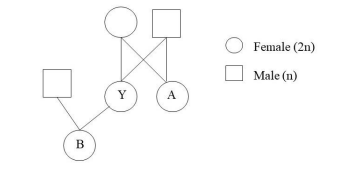
\includegraphics[]{figs/Q.63.png}
    \caption{}
    \label{fig:16}
\end{figure}

\hfill{(GATE EY 2023)}

%64

 \item Mixed species flocks of birds include social and solitary species. There are 5 social
species and 10 solitary species in a forest. Flocks always have a total of 5 species,
of which 2 are social and 3 are solitary. The number of types of flocks with unique
species composition is \underline{\hspace{1.5cm}}. (Answer in integer)
\hfill{(GATE EY 2023)}

%65


 \item In a zoo, three lions and four tigers eat 390 kg of food every week. In another zoo,
four lions and five tigers eat 500 kg of food every week. Lions and tigers eat
different amounts of food, but all individuals of the same species eat the same
amount. The amount of food a single lion eats per week is \underline{\hspace{1.5cm}} kg.
(Answer in integer)
\hfill{(GATE EY 2023)}


\begin{center}
    \textbf{END OF THE QUESTION PAPER}
\end{center}








    
\end{enumerate}

\end{document}
